\chapter{Principais Medidas Estatísticas}

\section{Introdução}

Algumas medidas de suma importância para a estatística são os somatórios e produtórios. Suas aplicabilidades vão desde a estatística descritiva, análise de variância, ao desenvolvimento de funções. Estes temas serão tratados a seguir.


\subsection{Somatório Simples}

\inic Muitos dos processos estatísticos exigem o cálculo da soma. Para simplificar a representação da operação de adição nas expressões algébricas, utiliza-se a notação representada pela letra grega sigma maiúsculo ($\Sigma$), na qual o somatório foi proposto para simplificar a representação da soma.\vskip0.3cm


Assim, $\sum_{i=1}^{n}x_{i}$  lê-se  somatório de x índice i, com i variando de 1 até n, em que n é a ordem da ultima parcela da soma ou o limite superior (LS) do somatório, i=1 é a ordem da primeira parcela da soma ou o limite inferior (LI), e i é o índice que está indexando os valores da variável  X (ou letras como Y, Z, W podem ser utilizadas).\vskip0.3cm

As letras do meio do alfabeto são geralmente usadas como índices, letras do final do alfabeto são comumente utilizadas como variáveis; e letras do inicio do alfabeto são freqüentemente empregadas para representar eventos em cálculo de probabilidades. Na verdade, o somatório nada mais é do que uma notação simplificada de várias somas.\vskip0.3cm

As principais representações dos somatórios são:


$$\sum_{i=1}^{n}x_{i}=x_{1}+x_{2}+\ldots+x_{n} \ \ Soma \ \ Simples$$

$$\sum_{i=1}^{n}x_{i}^{2}=x_{1}^{2}+x_{2}^{2}+\ldots+x_{n}^{2} \ \ Soma \ de \ Quadrados$$


$$ \left(\sum_{i=1}^{n}x_{i}\right)^{2}=(x_{i}+x_{2}+\ldots+x_{n})^{2} \ \ Quadrado \ da \ Soma$$

$$ \sum_{i=1}^{n}x_{i}y_{j}=(x_{1}y_{1}+x_{2}y_{2}+\ldots+x_{n}y_{n}) \ \ Soma \ de \ Produtos$$

$$ \sum_{i=1}^{n}x_{i} \sum_{j=1}^{m}y_{j}= (x_{1}+x_{2}+\ldots+x_{n})(y_{1}+y_{2}+\ldots+y_{n}) \ \ Produto \ da \ Soma$$


\subsection{Proriedades do Somatório}

\begin{enumerate}
  \item [{a})] O número de termos (NT) de um somatório refere-se à diferença entre os limites superior (ls) e inferior (li) acrescido da unidade, ou adicionalmente decrescido de r, quando o somatório estiver sujeito a r restrições.
\begin{equation}\label{}
    NT=(LS-LI)+1-r
\end{equation}
  \item [{b})] O somatório de uma constante k refere-se ao produto de NT por k.
$$\sum_{i=1}^{n}k=[(n-1)+1]k=nk$$
ou
$$ \sum_{i=1}^{n}k=k+k+\ldots+k=nk $$
  \item [{c})] O Somatório do produto de uma constante por uma variável que depende do somatório é igual ao produto da constate pelo somatório da variável, ou seja,
$$ \sum_{i=1}^{n}kx_{i}=kx_{1}+kx_{2}+\ldots+kx_{n}=k\sum_{i=1}^{n} $$
      \item [{d})] Propriedade Distributiva com relação à adição, isto é
$$ \sum_{i=1}^{n}(x_{i}+y_{j})= \sum_{i=1}^{n}x_{i}+ \sum_{i=1}^{n}y_{i} $$
  \item [{e})] Propriedade Distributiva com relação à subtração, isto é
$$ \sum_{i=1}^{n}(x_{i}-y_{j})= \sum_{i=1}^{n}x_{i}- \sum_{i=1}^{n}y_{i} $$
  \item [{f})] O Quadrado da soma é diferente da soma dos quadrados, ou seja,
  $$\left(\sum_{i=1}^{n}x_{i}\right)^{2}\neq \sum_{i=1}^{n}x_{i}^{2}$$
  \item [{g})] O Produto de duas somas é diferente da soma dos produtos, isto é
  $$ \sum_{i=1}^{n}x_{i} \times \sum_{i=1}^{n}y_{i} \neq \sum_{i=1}^{n} (x_{i} \times y_{i}) $$
  \item [{h})] O somatório de um quociente é diferente do quociente de duas somas.
$$ \sum_{i=1}^{n} \frac{x_{i}}{y_{i}} \neq \frac{\sum_{i=1}^{n}x_{i}}{\sum_{i=1}^{n}y_{i}}$$
  \item [{i})] O somatório duplo de um produto é igual ao produto dos somatórios tomados separadamente.
  $$  \sum_{i=1}^{n} \sum_{j=1}^{m}x_{i}y_{j}=  \sum_{i=1}^{n}x_{i} \times \sum_{j=1}^{m}y_{i}$$
\end{enumerate}


\subsection{Somatório Duplo}

Acontece com muita freqüência, na apresentação de dados estatísticos, o emprego de tabelas de dupla entrada, nas quais os valores são expressos em função de duas variáveis: uma variável linha e uma coluna. Desta maneira pode-se representar: estado civil (solteiro, casado, outros) versus o gênero (masculinoe feminino), as faixas etárias versus suas rendas, componentes versus modelos, etc. Assim, a indicação da soma dos elementos das tabelas de dupla entrada pode ser feita mediante o emprego do somatório duplo.\vskip0.3cm








\newpage

%\textbf{Exercícios de Somatório:}


%\begin{enumerate}
%  \item [{1)}] Sabe-se que: \\
%  $X_{1}=3$ $X_{2}=4$ $X_{3}=8$ $X_{4}=7$ $X_{5}=6$\\
%  $Y_{1}=3$ $Y_{2}=8$ $Y_{3}=2$ $Y_{4}=5$ $Y_{5}=6$\\
%  Calcule:
%  \begin{enumerate}
%    \item [{a)}] $\sum_{i=1}^{5}X_{i}$
%    \item [{b)}] $\sum_{i=1}^{5} 4 X_{i}$
%    \item [{c)}] $\sum_{i=3}^{5} (X_{i}+6)$
%    \item [{d)}] $\sum_{i=2}^{4} (2X_{i}-3)$
%    \item [{e)}] $\sum_{i=1}^{5}X_{i}Y_{i}$
%    \item [{f)}] $\sum_{i=1}^{5}(X_{i}+Y_{i})$
%  \end{enumerate}
%  \item [{2)}] Se o $\sum_{i=1}^{6}X_{i}=-4$ e %$\sum_{i=1}^{6}X_{i}^{2}=10$, calcular as seguintes expressões
%  \begin{enumerate}
%    \item [{a)}] $\sum_{i=1}^{6}(2X_{i}+3)$
%   \item [{b)}] $\sum_{i=1}^{6}(X_{i}-1)$
%   \item [{c)}] $\sum_{i=1}^{6}(X_{i}-5)^{2}$
%   \end{enumerate}
%  \item [{3)}] Dados $\sum_{i=1}^{4}X_{i}=7$, %$\sum_{i=1}^{4}Y_{i}=-3$ e $\sum_{i=1}^{4}X_{i}Y_{i}=5$, %determinar:
%  \begin{enumerate}
%    \item [{a)}] $\sum_{i=1}^{4}(2X_{i}+5X_{i})$
%    \item [{b)}] $\sum_{i=1}^{4}(X_{i}-3)(2Y_{i}+1)$
%   \end{enumerate}
%  \item [{4)}] Desenvolver os termos de cada uma das seguintes %somas indicadas:
%  \begin{enumerate}
%   \item [{a)}] $\sum_{i=1}^{n}a$
%    \item [{b)}] $ \sum_{i-1}^{6}X_{i}^{2}$
%    \item [{c)}] $\sum_{i=1}^{4}(Y_{1}-3)^{2} $
%    \item [{d)}] $\sum_{i=1}^{5}F_{i}X_{i} $
%    \item [{e)}] $\sum_{i=1}^{4}(X_{i}+Y_{i}) $
%    \item [{f)}] $\sum_{i=1}^{4}(\frac{X_{1}}{Y_{i}}-1)^{2} $
%    \item [{g)}] $\sum_{i=1}^{3}(X_{i}-a)$
%    \item [{h)}] $\sum_{i=1}^{5}f_{1}(Y_{i}-a)^{2}$
%  \end{enumerate}
%  \item [{5)}] Se $Z_{1}=X_{1}+Y_{1}$ e $Z_{2}=X_{2}+Y_{2} %\ldots Z_{n}=X_{n}+Y_{n}$, Provar que $\bar{Z}=\bar{X}+\bar{Y}$
%  \item [{6)}] Demonstrar que:
%  \begin{enumerate}
%    \item [{a)}] $\sum_{i=1}^{n}(X_{i}-\bar{X})=0$
%    \item [{b)}] $\sum_{i=1}^{n}(X_{i}-a)= Minimo$
%    \item [{c)}] $\sum_{i=1}^{n}X_{i}(X_{i}-%\bar{X})=\sum_{i=1}^{n}(X_{i}-\bar{X})^{2}$
%    \item [{d)}] $\sum_{i=1}^{n}[X_{1}(X_{i}+\bar{X})-%\bar{X}^{2}]=\sum_{i=1}^{n}X_{i=1}^{2}$
%    \item [{e)}] $\sum_{i=1}^{n}\sum_{j=1}^{n}(X_{i}-\bar{X})
%(Y_{j}-\bar{Y})=0$
%    \item [{f)}] $\sum_{i=1}^{n}[X_{i}(X_{i}+\bar{X})+(X_{i}-%\bar{X})^{2}]=2\sum_{j=1}^{n}X_{j}^{2}$
%    \item [{g)}] $\sum_{i=1}^{N}
%(X_{i}-1)^{2}=\sum_{i=1}^{N}X_{i}^{2}-2\sum_{i=1}^{N}+N$
%    \item [{h)}] $\sum f_{i}(x_{i}-\bar{x})^{2}= \sum %f_{i}x_{i}^{2}- \frac{(\sum f_{i}x_{i})^{2}}{\sum f_{i}}$
%  \end{enumerate}
%\end{enumerate}






\subsection{Produtório}

O símbolo produtório foi proposto para simplificar e facilitar a representação dos produtos nas expressões algébricas. Representado pela letra grega $pi$ maiúscula ($\Pi$).


\begin{equation}\label{}
    \prod_{i=1}^{n}x_{i}= x_{1} \times x_{2} \times  \ldots \times x_{n}
\end{equation}


Lê-se: produtório de X índice i, com i variando de 1 a n.

\vskip0.3cm

ou seja,

\begin{equation}\label{}
    \underbrace{x_{1} \times x_{2} \times  \ldots \times x_{n}}_{n fatores}= \prod_{i=1}^{n}x_{i}= x^{n}
\end{equation}









\subsection{Proporções e Percentagens}


Uma proporção é o número, $a$, de observações com determinada caracteristica (como por exemplo aqueles que sofreram um acidente de trânsito) dividido pelo número total de observações, $a+b$, num determinado grupo (como aqueles que estão na condição de Motociclistas). Isto é,


$$ 
\mbox{Proporção} = \left( \frac{a}{a+b} \right)
$$

Uma proporção sempre é definida como uma parte dividida pelo total e é útil para dados ordinais e números assim como para dados nominais, especialmente quando as observações forem colocadas numa tabela de frequência. Uma \textbf{Percentagem} é a proporção multiplicada por $100\%$.\vskip0.3cm


$$ \mbox{Proporção} = \left( \frac{a}{a+b} \right) \times 100\% $$

\newpage
\subsection{Razões}

Uma razão é o número $a$ de observações num determinado grupo com cada característica
dividida pelo número b de observações sem essa característica:


$$ 
\mbox{Razão} = \left( \frac{a}{b} \right)
$$

Uma razão sempre é definida como uma parte dividida por uma outra parte.\vskip0.3cm

\subsection{Taxas}

As Taxas são semelhantes as proporções exceto pelo fato de que é usado um multiplicador ($1.000 , 10.000 , ou 100.000$) e são calculados durante um período específico. O multiplicador é chamado de base e a fórmula é


$$ 
\mbox{Taxa} = \left( \frac{a}{a+b} \right) \times base
$$



\subsection{Coeficientes}

É a relação entre o número de eventos reais (os acontecimentos) e os esperados (que poderiam acontecer). È a medida de probabilidade. O numerador exprime o número de eventos ocorridos e o denominador exprime a população efetivamente exposta ao evento.\vskip0.3cm

Apresenta-se a seguir alguns exemplos de coeficientes.

\subsubsection{Coeficiente de Mortalidade Geral - CMG}

$$
C_{M_{G}} = \left(  \frac{numero \ de \ total \ de \ obitos \ em \ certa \ area \ durante \ o \ ano}{populacao \ da \ mesma \ area \ ajustada \ para \ o \ meio \ do \ ano} \right) \times 1.000
$$











\newpage
\section{Medidas de Tendência Central, Localização ou Posição}

Torna-se necessário, após a tabulação dos resultados e da representação gráfica, encontrar valores que possam representar a distribuição como um todo. São as chamadas medidas de tendência central, de posição ou localização.\vskip0.3cm

As medidas da tendência central são indicadores que permitem onde se tenha uma primeira idéia, um resumo, de como se distribuem os dados num experimento, informando o valor (ou faixa de valores) da variável aleatória que ocorre mais tipicamente, ou seja, compõem-se de um número que representa um conjunto particular de informações, geralmente, se localizam em torno do centro da distribuição, onde a maior parte das observações tende a concentrar-se.





\subsection{Média Aritmética Simples ($\bar{X}$)}

A média procura substituir um conjunto de valores por um valor só. Por isso
deve-se ter cuidado ao se interpretar uma média. Assim, quando se calcula uma média, esta se atribuindo
uma característica para a amostra em estudo.\vskip0.3cm

Vários tipos de medidas estatísticas podem ser definidas, sendo as mais comuns a \textbf{média}, \textbf{mediana}, \textbf{moda}, \textbf{média geométrica} e \textbf{harmônica}, apresentando vantagens e desvantagens
.\vskip0.3cm

Segundo FEIJOO (2010), a média aritmética representa o \textbf{centro de gravidade} da
distribuição, isto é, o ponto de qualquer distribuição em torno do qual se
equilibram as discrepâncias positivas e negativas. Situa-se entre o valor máximo e o valor mínimo da distribuição dos dados.\vskip0.3cm



%\begin{equation*}\label{media1}
%    \bar{X}=\frac{Soma \ Finita \ de \ Valores \ do \ Rol}{Quantidade \ de \ Termos \ que \ Compõem \ %os \ Dados}
%\end{equation*}



Sejam $x_{1}, x_{2}, ..., x_{n}$, os elementos de um rol numérico, valores particulares que a variável $x_{i} \in \mathbf{R}, (i=1,2,...,n), n \in \mathbf{N} $ assume, calcula-se a soma finita dos termos do numerador $(x_{1}+x_{2}+x_{3}+\ldots+x_{n})$,  pelo quociente do número total $(n_{1}+n_{2}+n_{3}+\ldots+n_{k})$ de termos que compõem o conjunto de dados.\vskip0.3cm


\begin{equation}\label{media1}
\bar{X}= \left[ \frac{x_{1}+x_{2}+x_{3}+\ldots+x_{n}}{n} \right ] = \left[ \frac{\sum_{i=1}^{n}x_{i}}{n} \right ]
\end{equation}


Para Hiebert e Lefevre (1986) e Gal (1995), os profissionais devem saber a utilidade da média, em que condições seu uso faz sentido, o que pode ocorrer se for utilizada inadequadamente, e reconhecer quando a média pode ser a melhor ferramenta ou quando Não deve ser usada.




%FEIJOO, AMLC. A pesquisa e a estatística na psicologia e na educação [online]. Rio de Janeiro:
%Centro Edelstein de Pesquisas Sociais, 2010, 109p. ISBN: 978-85-7982-048-9.

\newpage
\subsection{Média Aritmética Ponderada ($\bar{X}_{p}$)}

Seja $x$ uma variável que assume valores $x_{1},x_{2},\ldots,x_{n}$ com frequências absolutas respectivamente igual a $p_{1},p_{2},\ldots,p_{n}$. A média aritmética ponderada de $x$ é  definida como a divisão da soma de todos os produtos $x_{i} n_{i}(1,2,...,k)$ pela soma das frequências. Aplicando a equação \ref{media1}, temos que


$$
\Bar{x}_{1}=  \left[ \frac{x_{11},x_{12},\ldots, x_{1_{n_{1}}}}{n_{1}} \right ]
$$

$$
\Bar{x}_{2} =  \left[ \frac{x_{21},x_{22},\ldots, x_{2_{n_{2}}}}{n_{2}} \right ]
$$

$$
\vdots
$$

$$
\Bar{x}_{k} = \left[ \frac{x_{k1},x_{k2},\ldots, x_{k_{n_{k}}}}{n_{k}}  \right ]
$$

com isso, 

$$
p_{1}\Bar{x}_{1} = [x_{11},x_{12},\ldots, x_{1_{p_{1}}}]
$$

$$
p_{2}\Bar{x}_{2} = [x_{21},x_{22},\ldots, x_{2_{p_{2}}}]
$$

$$
\vdots
$$

$$
p_{k}\Bar{x}_{k} = [x_{k1},x_{k2},\ldots, x_{k_{p_{k}}}]
$$

Assim, a média aritmética de todos os números é:

$$
\Bar{x} = \left[ \frac{(x_{11},x_{12}+\ldots+x_{1_{n_{1}}})+(x_{21}+x_{22}+\ldots+x_{2_{n_{2}}})+(x_{k_{1}}+x_{k_{2}}+\ldots+x_{k_{n_{k}}})}{p_{1}+p_{2}+\ldots+p_{k}} \right ]
$$


logo a expressão é equivalente a

\begin{equation}\label{media}
    \bar{X} =  \left[ \frac{(p_{1}\Bar{x}_{1})+(p_{2}\Bar{x}_{2})+\ldots+(p_{k}\Bar{x}_{k})}{p_{1}+p_{2}+\ldots+p_{k}} \right ]  =   \left[ \frac{\sum_{i=1}^{n}x_{i}p_{i}}{\sum_{i=1}^{n}p_{i}} \right ]
\end{equation}







\newpage
\subsection{Propriedades da Média Aritmética}

A média aritmética possui as seguintes propriedades (SILVA, 2011), (SPIGEL et al, 2013), (IEZZY et al, 2013) e (Bussab e Morettin 2017). 

\begin{enumerate}
\item [{A)}] A média aritmética de uma \textbf{constante} é a própria constante.

\vskip0.3cm
\textbf{\fbox{Provar para constante $c$:}} 

Sejam  $x_{1}=b, x_{2}=b, ..., x_{n}=b$, por definição da média aritimética conforme a equação \ref{media1} tem-se que: $x_{1}=x_{2}=,..., x_{n}=b$, então a expressão \ref{media1} equivale a

\begin{equation*}\label{propriedade1}
\bar{x} = \left[ \frac{b+b+...+b}{n} \right ] = \left [\frac{nb}{n} \right ]= b
\end{equation*}
 

\item [{B)}] A média aritmética é um valor contido entre o menor e o maior valor observado; 

\vskip0.3cm
\textbf{\fbox{Provar para $x_{i} \leq \Bar{x}:$}} 

Seja a sequência de números reais $x_{1},x_{2},x_{i},x_{j},\ldots,x_{n}$ com $x_{i}$= mínimo da sequência e $x_{n}$= máximo da sequência. \vskip0.3cm

Pela definição da equação \ref{media1}, $x_{i}$ é o mínimo da sequência, então 

\begin{equation*}\label{propriedade1}
x_{i}+x_{i}+x_{i}+\ldots+x_{i} \leq  x_{1}+x_{2}+x_{3}+\ldots+x_{n}
\end{equation*}

Devido,

\begin{equation*}\label{propriedade1}
x_{1}+x_{2}+x_{3}+\ldots+x_{n}=n \Bar{x}
\end{equation*}

Logo, a expressão

\begin{equation*}\label{propriedade1}
x_{i}+x_{i}+x_{i}+\ldots+x_{i} \leq n \Bar{x}
\end{equation*}

que é equivalente a 

\begin{equation*}\label{propriedade1}
\left[ \frac{x_{i}+x_{i}+x_{i}+\ldots+x_{i}}{n}  \right ] \leq \Bar{x}
\end{equation*}

que equivale a 

\begin{equation*}\label{propriedade1}
\left[ \frac{nx_{i}}{n} \right ]  \leq \Bar{x}
\end{equation*}

Logo,

\begin{equation*}\label{propriedade1}
x_{i} \leq \Bar{x}
\end{equation*}

Portanto, a média aritmética é maior ou igual que o mínimo da sequência.



\vskip0.3cm
\textbf{\fbox{Provar para $x_{n} \geq  \Bar{x}:}}$
\vskip0.3cm

Seja a sequência de números reais $x_{1},x_{2},x_{i},x_{j},\ldots,x_{n}$ com $x_{i}$= mínimo da sequência e $x_{n}$= máximo da sequência. \vskip0.3cm

Pela definição da equação \ref{media1}, $x_{i}$ é o máximo da sequência, então 

\begin{equation*}\label{propriedade1}
x_{i}+x_{i}+x_{i}+\ldots+x_{i} \geq  x_{1}+x_{2}+x_{3}+\ldots+x_{n}
\end{equation*}

Devido,

\begin{equation*}\label{propriedade1}
x_{1}+x_{2}+x_{3}+\ldots+x_{n}=n \Bar{x}
\end{equation*}

Logo, a expressão

\begin{equation*}\label{propriedade1}
x_{i}+x_{i}+x_{i}+\ldots+x_{i} \geq n \Bar{x}
\end{equation*}

que é equivalente a 

\begin{equation*}\label{propriedade1}
\left[ \frac{x_{i}+x_{i}+x_{i}+\ldots+x_{i}}{n} \right ] \geq \Bar{x}
\end{equation*}

que equivale a 

\begin{equation*}\label{propriedade1}
\left[ \frac{n \times x_{n}}{n} \right ] \geq \Bar{x}
\end{equation*}

Logo,

\begin{equation*}\label{propriedade1}
x_{n} \geq \Bar{x}
\end{equation*}

Portanto, a média aritmética é menor ou igual que o máximo da sequência.



\item [{C)}] A soma algébrica dos desvios de um conjunto de números em relação a média é sempre zero.\vskip0.3cm

Quando se trabalha com dados brutos.
$$ \sum_{i=1}^{n}(x_{i}-\bar{X})=0 $$


Quando se trabalha com dados tabulados.
$$ \sum_{i=1}^{n}f_{i}[(x_{i}-\bar{X})]=0 $$



\textbf{\fbox{Provar para Dados Brutos:}} 
\vskip0.3cm

Seja a sequência  $x_{1}+x_{2}+x_{3}+\ldots+x_{n}$ de média aritmética $\Bar{x}$, então o desvio $d_{i}$ do elemento $x_{i}$, com $1=1,2,3,\ldots,n$ é dado por $d_{i}=x_{i}-\Bar{x}$.
\vskip0.3cm


Assim, 

\begin{eqnarray*}
= & (x_{1}-\Bar{x})+(x_{2}-\Bar{x}_{1})+(x_{3}-\Bar{x}_{2})+\ldots+(x_{n}-\Bar{x}_{n}) \\
= & (x_{1}+x_{2}+x_{3}+\ldots+x_{n}) - (\Bar{x}_{1}-\Bar{x}_{2}+\Bar{x}_{3}+\ldots+\Bar{x}_{n})\\
= & (x_{1}+x_{2}+x_{3}+\ldots+x_{n})-(n\Bar{x})\\
= & (x_{1}+x_{2}+x_{3}+\ldots+x_{n})-n \left(\frac{(x_{1}+x_{2}+x_{3}+\ldots+x_{n})}{n} \right)\\
= & (x_{1}+x_{2}+x_{3}+\ldots+x_{n})-(x_{1}+x_{2}+x_{3}+\ldots+x_{n})\\
= & (x_{1}+x_{2}+x_{3}+\ldots+x_{n})-(x_{1}-x_{2}-x_{3}-\ldots-x_{n})\\
= & (x_{1}-x_{1})+(x_{2}-x_{2})+(x_{3}-x_{3})+(\ldots)+(x_{n}-x_{n})\\
= & 0+0+0+\ldots+0=0
\end{eqnarray*}

Nesse contexto, a Soma dos desvios tomados em relação a média aritmética é zero.




\newpage

\item [{D)}] A soma dos quadrados dos desvios de um conjunto de números, em relação a qualquer número $a$, é um mínimo quando a é igual a média e somente neste caso.\vskip0.3cm
Quando se trabalha com dados brutos.

$$ \sum_{i=1}^{n}(x_{i}- a)= Minimo  $$
Quando se trabalha com dados tabulados.
$$ \sum_{i=1}^{n}f_{i}[(x_{i}- a)]= Minimo  $$

  \item [{E)}] Multiplicando-se (ou Dividindo-se) todos os elementos
de um conjunto de dados por uma \textbf{constante}, média aritimética fica multiplicada ou dividida por essa constante;

\vskip0.3cm
\textbf{\fbox{Provar para Multiplicação:}} 
\vskip0.3cm

Sejam sequência de números reais $x_{1}, x_{2},...,x_{n}$ os valores assumidos por uma variável $x$ e $\Bar{x}$ a média aritmética correspondente. Se a cada $(x_{i}=1,2,...,n)$, multiplicar uma \textbf{constante real c}, a média aritmética fica multiplicada de \textbf{c} unidades.\vskip0.3cm


Considera-se que os novos valores assumidos por essa variável sejam: 

$$(c_{1}x_{1}),(c_{2}x_{2}),...,(c_{n}x_{n})$$

a nova média é dada por:

\begin{equation*}\label{media3}
     \bar{x} =  \left[ \frac{(c_{1}x_{1})+(c_{2}x{2})+(c_{3}x{3})+\ldots+(c_{n}x{n})}{n} \right]
\end{equation*}

\begin{equation*}\label{media3}
     \bar{x} = \left[ \frac{c(x_{1}+x_{2}+x_{3}+\ldots+x_{n})}{n} \right]
\end{equation*}

\begin{equation*}\label{media3}
     \bar{x}=c \left[\frac{(x_{1}+x_{2}+x_{3}+\ldots+x_{n})}{n} \right]
\end{equation*}


\begin{equation*}\label{media3}
     \bar{x}=c_{i}\Bar{x} 
\end{equation*}



\vskip0.3cm
\textbf{\fbox{Provar para Divisão:}} 
\vskip0.3cm

Sejam sequência de números reais $x_{1}, x_{2},...,x_{n}$ os valores assumidos por uma variável $x$ e $\Bar{x}$ a média aritmética correspondente. Se a cada $(x_{i}=1,2,...,n)$, dividir uma \textbf{constante real c}, a média aritmética fica multiplicada de \textbf{c} unidades.\vskip0.3cm


Considera-se que os novos valores assumidos por essa variável sejam: 

$$\left( \frac{x_{1}}{c_{1}} \right), \left( \frac{x_{2}}{c_{2}} \right),..., \left( \frac{x_{n}}{c_{n}}\right)$$


a nova média é dada por:

\begin{equation*}\label{media3}
     \bar{x} = \left[ \frac{\left( \frac{x_{1}}{c_{1}} \right)+ \left( \frac{x_{2}}{c_{2}} \right)+ \left( \frac{x_{3}}{c_{3}}\right)+\ldots+\left( \frac{x_{n}}{c_{n}} \right)}{n} \right]
\end{equation*}

\begin{equation*}\label{media3}
     \bar{x}= \left[ \frac{ \frac{1}{c} \left( x_{1}+x_{2}+x_{3}+\ldots+x_{n} \right)}{n} \right]
\end{equation*}

\begin{equation*}\label{media3}
     \bar{x}= \frac{1}{c} \left[ \frac{x_{1}+x_{2}+x_{3}+\ldots+x_{n}}{n} \right]
\end{equation*}

\begin{equation*}\label{media3}
     \bar{x}= \left[ \frac{\bar{x}}{c_{i}} \right]
\end{equation*}

Com isso, a média aritmética sofreu a mesma operação que os valores de $x_{i}$.

\item [{F)}] Somando-se (ou subtraindo-se) uma constante positiva de todos os elementos de um conjunto de dados, a média aritmética fica aumentada (ou diminuída) dessa constante;

%\vskip0.3cm
\newpage
\textbf{\fbox{Provar para Soma:}} 
\vskip0.3cm

Sejam $x_{1}, x_{2},...,x_{n}$ os valores assumidos por uma variável $x$ e $\Bar{x}$ a média aritmética correspondente. Se a cada $(x_{i}=1,2,...,n)$, adiciornar uma \textbf{constante real c}, a média aritmética fica adicionada de \textbf{c} unidades.\vskip0.3cm

Considera-se que os novos valores assumidos por essa variável sejam: $(x_{1}+c),(x_{2}+c),...,(x_{n}+c)$, a nova média é dada por:

\begin{equation*}\label{media3}
     \bar{x} = \left[ \frac{\sum_{i=1}^{n}(x_{i}+c)}{n} \right] =  \left[  \frac{(x_{1}+c)+(x_{2}+c)+...+(x_{n}+c)}{n} \right]
\end{equation*}

\begin{equation*}\label{media4}
  = \left[ \frac{(x_{1})+(x_{2})+...+(x_{n})}{n} \right] +  \left[ \overbrace{\frac{c+c+...+c}{n}}^{n} \right]+ 
 \left[ \frac{\sum_{i=1}^{n}x_{i}}{n}\right] = \left[ \frac{n \times c}{c} \right]
\end{equation*}

isto é, 

$$\Bar{x}^{'}=\Bar{x}+c$$



\vskip0.3cm
\textbf{\fbox{Provar para Subtração:}} 
\vskip0.3cm

Sejam $x_{1}, x_{2},...,x_{n}$ os valores assumidos por uma variável $x$ e $\Bar{x}$ a média aritmética correspondente. Se a cada $(x_{i}=1,2,...,n)$, subtrair uma \textbf{constante real c}, a média aritmética fica adicionada de \textbf{c} unidades.\vskip0.3cm


Considera-se que os novos valores assumidos por essa variável sejam: $(x_{1}-c),(x_{2}-c),...,(x_{n}-c)$, a nova média é dada por:

\begin{equation}\label{media3}
     \bar{x} = \left[ \frac{\sum_{i=1}^{n}(x_{i}-c)}{n} \right] = \left[ \frac{(x_{1}-c)+(x_{2}-c)+...+(x_{n}-c)}{n} \right] 
\end{equation}

\begin{equation*}\label{media4}
  = \left[ \frac{(x_{1})+(x_{2})+...+(x_{n})}{n} \right] - \left[ \overbrace{\frac{c-c-...-c}{n}}^{n} \right] + \left[ \frac{\sum_{i=1}^{n}x_{i}}{n} \right] = \left[ - \frac{n \times c}{c} \right]
\end{equation*}

isto é, 

$$\Bar{x}^{'}=\Bar{x}-c$$




\item [{G)}]Multiplicando-se todas as frequências de uma distribuição por uma constante positiva, a média aritmética não se autera; 
\end{enumerate}



%\item[{H)}] 












\subsection{Média Artimética(Dados Tabulados)}

Se os números $x_{1},x_{2},x_{3},\ldots, x_{n}$ ocorrerem $f_{1}, f_{2}, f_{3}, \ldots, f_{n}$ vezes, a média aritmética para dados em tabelas será:


\begin{equation}\label{media2}
     \bar{X}= \left[ \frac{x_{1}f_{1}+x_{2}f_{2}+x_{3}f_{3}+
 \ldots+x_{n}f_{n}}{f_{1}+f_{2}+f_{3}+\ldots+f_{n}} \right ]=   \left[\frac{\sum_{i=1}^{n}f_{i}x_{i}}{\sum_{i=1}^{n}f_{i}} \right ]
\end{equation}

\subsection{Média Geométrica Simples ($\bar{X}_{g}$)}

Quando uma variável tende a crescer ou drescrecer geometricamente, recomenda-se o uso da média geométrica, que é definida como sendo a rais n-ésima do produto dos n valores sa série observada. Ao contrário da média aritmética, a média geométrica não é muito influênciada pelos valores extremos de uma seuqência numérica.\vskip0.3cm


A média geométrica (G) de um conjunto de números $X_{1},X_{2},\ldots,X_{N}$ é a raiz de ordem n do produto
desses números:

\begin{equation}\label{Geometrica}
    G=\sqrt[n]{X_{1},X_{2},\ldots,X_{N}}=\sqrt[n]{\coprod_{i=1}^{n}X_{i}}
\end{equation}


\subsection{Média Geométrica Ponderada ($\Bar{X}_{g_{p}})$}

A média geométrica ponderada é semelhante à média geométrica. A diferença básica é que cada um dos seus elementos pode ser influenciado por multiplicador denominado de peso, enquanto na média geométrica cada um dos elementos tem multiplicador unitário, omitido.\vskip0.3cm


Sejam os números $X_{1},X_{2},\ldots,X_{k}$ ocorrem com frequências $f_{1},f_{2},\ldots,f_{k}$, sendo $f_{1},f_{2},\ldots,f_{k}=N$, frequência total.


\begin{equation}\label{Geometrica}
    G=\sqrt[n]{\underbrace{X_{1},X_{1},...,X_{1}}_{f_{1vezes}}\underbrace{X_{2},X_{2},...,X_{2}}_{f_{2vezes}} \ldots \underbrace{X_{k},X_{k},...,X_{k}}_{f_{kvezes}}}=\sqrt[n]{X_{1}^{f_{1}}X_{2}^{f_{2}}\ldots X_{k}^{f_{k}}}
 = \sqrt[\sum f_{i}]{\coprod_{i=1}^{n}X_{i}}
\end{equation}

Essa expressão é conhecida como média geométrica ponderada.



\subsection{Média Harmônica Simples ($\bar{X}_{h})$}


\inic Um terceiro tipo de média, também sem grande interesse no estudo das
distribuições de frequências, mas que é de grande utilidade em situações em que não
tem lógica adicionar valores da amostra, é o de média harmónica.\vskip0.3cm



È utilizada quando os fenômenos envolvidos variam de forma inversamente proporcional a outros considerados.\vskip0.3cm

\textbf{Exemplos}:
\begin{enumerate}
  \item Na bolsa de valores, onde a média aritmética das cotações de títulos deve corresponer a média harmônica das taxas de juros do mercado;
  \item Nas populações, onde a média aritmética da taxa de mortalidade corresponde a média harmônica da duração de vida;
\end{enumerate}

Onde a média harmônica dá mais importância aos valores menores da distribuição, e não é definida, quando pelo menos um valor da série for nulo.\vskip0.3cm


A média harmônica de um conjunto de números $x_{1},x_{2},\ldots,x_{n}$ é a inverso da média
aritmética das recíprocas dos números, ou seja,


\begin{equation}\label{harmonica1}
H= \left[ \frac{  (\frac{1}{x_{1}})+(\frac{1}{x_{2}})+\ldots+(\frac{1}{x_{n}})  }{n} \right ]  ^{-1} 
\end{equation}

\begin{equation*}\label{harmonica1}
 =\left[  \frac{n}{\frac{1}{X_{1}}+\frac{1}{X_{2}}+\ldots+\frac{1}{X_{n}}}  \right ]
\end{equation*}

\begin{equation*}\label{harmonica}
=\left[  \frac{1}{\frac{1}{N}\sum_{i=1}^{n}\frac{1}{X_{i}}} \right ]
\end{equation*}

\vskip0.3cm

\textbf{Exemplor Prático}: Os Agentes de Fiscalização de Trânsito do DETRAN-PA, fazem o acompanhamento tático da imagem de Nossa senhora de Nazaré durante o mês de outubro (\textbf{Círio de Nazaré}). Viajando de Belém para Marituba à velocidade média de 30 km/h e volta de Marituba para Belém, pelo mesmo caminho, à velocidade média de 60 km/h. Qual a velocidade média para a viagem completa.

\begin{equation}\label{exemplo_harmonica}
Velocidade \ \  Media = \left[\frac{2}{\frac{1}{30}+\frac{1}{60}} \right ]= 40 km/h
\end{equation}


\subsection{Média Harmônica Ponderada ($\bar{X}_{h_{p}})$}


Se os dados estiverem agrupados sob a forma de distribuição por classe de valores, a média harmônica podenrada será:


\begin{equation}\label{harmonicapondrada}
    \bar{X}_{H}= \left[  \frac{\sum_{i=1}^{n}p_{i}}{\frac{p_{1}}{X_{1}}+\frac{p_{2}}{X_{2}}+\ldots+\frac{p_{n}}{X_{n}}}\right ] = \left[  \frac{\sum_{i=1}^{n}p_{i}}{\sum_{i=1}^{n}\frac{p_{i}}{x_{i}}} \right ]
\end{equation}


A relação entre a média geométrica, harmônica e a aritmética, pode ser representada da seguinte forma:

        $$ H \leq G \leq \bar{X}  $$

A média Geométrica de um conjunto de números positivos $X_{1},X_{2},\ldots,X_{N}$ é menor do que ou igual a sua média aritmética, mas é maior do que ou igual a sua média harmônica.


\subsection{Média Aparada ($\bar{X}_{tm}$)}


\inic Como se referiu ao introduzir a noção de média aritmética, esta tem especial
importância no estudo das distribuições de frequências.
Acontece, como facilmente pode comprovar-se, que se trata de um conceito
pouco flexível, e fortemente influenciado pelos valores extremos que possam surgir na
amostra. Com a finalidade de evitar os efeitos desaconselháveis de possíveis valores
extravagantes, recorre-se ao conceito de média aparada. \vskip0.3cm


A média aparada (\textbf{trimmed mean}) é uma medida de localização resistente, cuja sensibilidade a pontos aberrantes ou chamados outliers, é reduzida por remover uma proporção especificada da observação maior e menor, ou seja, elimina os valores extremos. Se a proporção de observações omitida de cada lado é $\alpha$, então a média dos $\alpha$ dados cortados é dada por:

\begin{equation}\label{aparada}
    \bar{X}_{\alpha} = \left[\frac{1}{n-2k} \right] \sum_{i=k+1}^{n-k}X_{i}
\end{equation}

Onde k é o valor inteiro arredondado do produto $\alpha n$, o número de valores de dados "cortados" de cada cauda. A média aparada reduz-se à média aritmética quando $\alpha = 0$.


\subsection{Mediana $(\widetilde{X})$}


\inic Outra estatística usada para indicar o centro de um conjunto de dados é a mediana amostral, que pode ser definida, de maneira simplificada como o valor intermediário do conjunto de dados, cujos n valores são dispostos ordenadamente.\vskip0.3cm


A mediana algumas vezes é simbolizada por $M$ ou $Md$, mas não possui um símbolo convencional.\vskip0.3cm



A mediana é uma medida de posição indicada quando o conjunto de dados possui valores extremos,
o que pode comprometer a discussão dos dados baseados simplesmente na média, ou seja, é o
valor central em um rol de valores que divide a distribuição ao meio, correspondendo a 50\% dos dados.\vskip0.3cm

Sendo que existem duas formas de se calcular uma mediana: quando os dados são brutos ou em forma de tabelas.\vskip0.3cm


\subsection{Mediana de Valores Brutos}


\begin{enumerate}
  \item Primeiramente, para se calcular a mediana é ordenar os valores em ordem crescente (Rol);
  \item Se o n (número total de elementos) for Ímpar, a mediana será o valor central;
  \item Se o n (número total de elementos) for Par, o conjunto terá dois valores centrais, neste caso, a mediana será igual à média aritmética dos valores centrais;
\end{enumerate}

\subsection{Mediana de Valores Tabelados}


Para valores agrupados em classes de frequência, a mediana será calculada através de uma fórmula, ou por interpolação da ogiva de galton, utilizando os seguintes passos.



\begin{enumerate}
\item [{1°)}] Completar a tabela criando a coluna para as frequências acumulada, caso não haja essa coluna;
\item [{2°)}]Identificar a classe da mediana, procurando o elemento que ocupa a posição.
$$ P_{i} = \left[\frac{\sum_{i=1}^{n}f_{i}}{2} \right]  $$
\item [{3°)}] Posteriormente, marca-se na tabela a posição, para identificar em qual classe estará a mediana.
\item [{4°)}] Em seguida aplica-se a fórmula da mediana
\end{enumerate}

\begin{equation}\label{}
    \tilde{X}(Me)=l_{i}+\left[\frac{P-FAA}{f_{i}}\right]\times h_{i}
\end{equation}

 onde

 \begin{itemize}
   \item $l_{i}=$ é o limite inferior da classe que contém a mediana;
   \item $FAA=$ é a frequência acumulada anterior à classe da mediana;
   \item $f_{i}=$ é a frequência simples da classe da mediana;
   \item $h_{i}=$ é a amplitude da classe que comtém a mediana;
 \end{itemize}


Geometricamente, a mediana é o valor de X (abscissa) correspondente a vertical que divide o histograma em duas partes de áreas iguais.\vskip0.3cm


(EXEMPLO) Utilizando as notas referentes a disciplina de estatística aplicada ministrada aos alunos do curso de engenharia civil matriculados na UFPA em 2022 para demostração do uso do cálculo da mediana.



  \begin{table}[!htb]
    \centering
    {
    \caption{Notas da Disciplina de Estatistica Aplicada dos Alunos de Engenharia Civil na UFPA em 2022.}
    \label{exemplomediana}
    \vspace{0.1cm}
\begin{tabular}{l|c|c}
  \hline\hline
  Notas          & Frequência Simples & Frequência Acumulada \\
  \hline\hline
  $0 \vdash 2  $ & 4          & 4                    \\
  $2 \vdash 4  $ & 12         & 16                   \\
  $4 \vdash 6  $ & 15         & 31                   \\
  $6 \vdash 8  $ & 13         & 44                   \\
  $8 \vdash 10 $ & 6          & 50                   \\
  \hline\hline
  Total & 50                  &  - \\
    \hline\hline
\end{tabular}}
\end{table}

$1° \mbox{\textbf{Passo}}:$ Inicialmente vamos completar a tabela criando a coluna para as frequências acumuladas.\vskip0.3cm

$2° \mbox{\textbf{Passo}}:$ Identificar a classe da mediana, procurando o elemento que ocupa a seguinte posição

$$ P= \left[ \frac{n}{2} \right] = \left[ \frac{50}{2} \right] = 25 $$

O 25° elemento, se encontra na classe 3, portanto a mediana se encontra o intervalo $ 4 \vdash 6$.

\vskip0.3cm

$3° \mbox{\textbf{Passo}}:$ Identificar os elementos relativos a classe mediana:

\begin{itemize}
  \item Limite Inferior da classe que contém a mediana ($l_{inf}=4$);
  \item Frequência Acumulada anterior a classe da mediana ($FAA=16$)
  \item Frequência Simples da classe da mediana ($f_{1}=15$)
  \item Amplitude da classe que contém a mediana ($h_{1}=2$)
\end{itemize}

$4° \mbox{\textbf{Passo}}:$ Calcular a Mediana aplicando a fórmula


\begin{equation}\label{}
    \tilde{X}(Me)= 4+\left[\frac{25-16}{15}\right]\times 2 = 5,2
\end{equation}








\subsection{Propriedades da Mediana}

A mediana possui algumas propriedades (SILVA, 2011) e (SPIGEL et al, 2013).

\begin{itemize}
\item A mediana pode ou não coincidir com um elemento da série;
\item A mediana pode ou não coincidir com amédia artimética;
\item A contrário da média, a mediana não sofre a influencia de valores extremos, pois depende da posição e não dos valores dos elementos da série. Por causa dessa característica, em muitos casos, ou da mediana é mais conveniente que a média.    
\end{itemize}


Do ponto de vista visual, é fácil determinar a mediana a partir de um gráfico chamado \textbf{Ramos e Folhas} das observações.




\subsection{Moda (M_{o})}

A moda é aquilo que esta em evidência, o valor que mais aparece num conjunto de informações ou o de maior freqüência em uma tabela. Em outras palavras, a moda tem a maior probabilidade de aocorrer. Sendo que a moda pode não ser única ou até mesmo pode não existir (SPIGEL et al, 2013).\vskip0.3cm


Sendo que existem duas formas de se calcular uma moda: quando os dados são brutos ou em forma de tabelas.\vskip0.3cm

É relevante salientar que um conjunto de dados pode apresentar todos seus elementos com a mesma freqüência absoluta, e neste caso não existirá um valor modal, o que significa que a distribuição será classificada como amodal.\vskip0.3cm

\textbf{Exemplo:} Na sequência 1,1,3,3,4,4, todos elementos apresentam frequência 2, logo a sequência é \textbf{Amodal} (sem moda).\vskip0.3cm

Quando uma sequência de valores apresenta uma moda, classifica-se que a distribuição é \textbf{Unimodal}.\vskip0.3cm


\textbf{Exemplo:} Na sequência 6,6,9,10,10,11,12,14,15, o elemento de valor 10, aprensenta frequência 3, que é a maior frequência entre os elementos, logo a distribuição é \textbf{unimodal} e a moda é 10.\vskip0.3cm

Podem ocorrer, também, casos em que a seqüência de observações apresente dois elementos com freqüência iguais, implicando numa distribuição \textbf{Bimodal}, e situações em que vários elementos com quantidade iguais, sendo chamada de distribuição \textbf{Polimodal, Plurimodal ou multimodal}.\vskip0.3cm

O uso da moda é mais indicado quando se deseja obter, rapidamente, uma medida de tendência central. Outro aspecto que favorece a utilização da moda é que seu valor não é afetado pelos valores extremos do conjunto de dados analisado.\vskip0.3cm

\subsection{Moda de Valores Brutos}

%\textbf{Moda de Valores Brutos}
\vskip0.3cm


É o ponto médio da classe que contém, a moda. Trata-se de um cálculo bruto, sem precisão.

\begin{equation}\label{}
    M_{0}= \left[\frac{l_{mo}+L_{mo}}{2}\right]
\end{equation}


\subsection{Moda de Valores Tabulados}

%\textbf{Moda de Valores Tabelados}
\vskip0.3cm

Para valores agrupados em classes de frequência, a moda será calculada através de fórmulas, ou por interpolação linear. Teremos a moda de valores tabelados, calculadas pelas fórmulas de KING e CZUBER.
\vskip0.3cm


\textbf{Moda pelo Método de King}
\vskip0.3cm

A moda via fórmula de King, é menos precisa do que a moda de Czuber, seu cálculo será feito pela seguinte fórmula.


\begin{equation}\label{}
    Mo=l_{mo}+\left[\frac{f_{mo}}{f_{ant}+f_{post}}\right]\times h_{i}
\end{equation}


%\newpage
\textbf{Moda pelo Método de Czuber}
\vskip0.3cm

A fórmula de czuber apresenta o valor mais preciso para o calculo da moda. Vejamos os procedimentos
de cálculo da moda de uma distribuição pela fórmula de czuber.


\begin{enumerate}
\item [{1°)}] Determinar a classe modal (de maior frequência simples) e o limite inferior ($l_{i}$) do intervalo que representa a classe da moda;
\item [{2°)}] Identificar esses elementos
\begin{itemize}
   \item $f_{mo}=$ é a frequência simples da classe modal;
   \item $f_{ant}=$ é a frequência simples da classe anterior a modal;
   \item $f_{post}=$ é a frequência simples da classe posterior a modal;
   \item $h_{i}=$ é a amplitude do intervalo da classe modal;
 \end{itemize}
\item [{4°)}] Em seguida usa-se a fórmula de czuber.
\end{enumerate}

\begin{equation}\label{}
    Mo=l_{i}+\left[\frac{f_{mo}-f_{ant}}{2f_{mo}-(f_{ant}-f_{post})}\right]\times h_{i}
\end{equation}





%\newpage

%\subsection{Exercícios Aplicados em Concursos (média-moda-mediana)}


%\begin{enumerate}
%  \item [{1)}] (\textbf{BACEN-1994}) Em certa Empresa W, o salário %médio era de R\$9.000,00 e o desvio-padrão dos salários era de
%  R\$ 1.000,00. Todos os salários receberam um aumento de 10\%. O %salário médio passou a ser de:\vskip0.3cm
%  \begin{itemize}
%    \item [{a)}] R\$ 9.000,00
%    \item [{b)}] R\$ 9.100,00
%    \item [{c)}] R\$ 9.500,00
%    \item [{d)}] R\$ 9.900,00
%    \item [{e)}] R\$ 10.000,00
%  \end{itemize}
%  \item [{2)}] Em um concurso realizado simultaneamente nas cidades %A, B e C, as médias aritméticas foram respectivamente 70, 60 e 45 %pontos, obtidas por 30, 40 e 30 candidatos, na mesma prdem. Qual foi %então a média aritmética geral do concurso?
%      \begin{itemize}
%    \item [{a)}] 60,0
%    \item [{b)}] 75,5
%    \item [{c)}] 58,5
%    \item [{d)}] 180
%    \item [{e)}] 682
%  \end{itemize}
%  \item [{3)}] Sabe-se que a média aritimética de 5 números inteiros %distintos, estritamente positivos, é 16. O maior valor que um desses %inteiros pode assumir é:
%  \begin{itemize}
%    \item [{a)}] 16
%    \item [{b)}] 20
%    \item [{c)}] 50
%    \item [{d)}] 70
%   \item [{e)}] 100
%  \end{itemize}
%  \item [{4)}](\textbf{GDF-1995}) Os preços do $m^{2}$ das ultimas %cinco obras realizadas por uma instituição pública foram %respectivamente: 800, 810, 810, 750 e 780 URV'S. Pode-se afirmar que %a média dos preços do $m^{2}$ obtido é:
%  \begin{itemize}
%    \item [{a)}] 780
%    \item [{b)}] 790
%    \item [{c)}] 800
%    \item [{d)}] 810
%  \end{itemize}
%  \item [{5)}](\textbf{TTN-1985}) Assinale a alternativa correta, %considerando a série;8;5;14;10;8 e 15
%  \begin{itemize}
%    \item [{a)}] A média aritmética é 10 e a mediana é 12;
%    \item [{b)}] A amplitude total é 7 e a moda é 8;
%    \item [{c)}] A mediana é 9 e a amplitude total é 10;
%    \item [{d)}] A média aritmética é 1 e a amplitude total é 7;
%    \item [{e)}] A mediana é 12 e a amplitude total é 7;
%  \end{itemize}
%  \item [{6)}](\textbf{TTN-1994}) A distribuição dos salários de uma %Empresa Y é dada na tabela abaixo:
%  \begin{table}[!htb]
%    \centering
%    {
%    \caption{Distribuição Salarial dos funcionários da empresa Y em %1994}
%    \label{}
%    \vspace{0.1cm}
%\begin{tabular}{l|c}
%  \hline\hline
%  Salário (em R\$) & Número de Empregados \\
%  \hline\hline
%   500,00    & 10 \\
%   1.000,00  & 5 \\
%   1.500,00  & 1 \\
%   2.000,00  & 10 \\
%   5.000,00  & 4 \\
%   10.500,00 & 1 \\
%  \hline\hline
%  Total & 31 \\
%    \hline\hline
%\end{tabular}}
%\end{table}
%\inic O salário modal, a média e a mediana dos salários dessa %empresa valem, respectivamente:
%  \begin{itemize}
%    \item [{a)}] 2.000,00 e 1.500,00; 500,00 e 1.000,00
%    \item [{b)}] 1.500,00 e 2.000,00; 1.500,00 e 2.000,00
%    \item [{c)}] 2.000,00 e 2.000,00; 2.000,00 e 2.000,00
%    \item [{d)}] 1.500,00 e 1.500,00; 1.500,00 e 1.500,00
%    \item [{e)}] 500,00 e 2.000,00; 2.000,00 e 1.500,00
%  \end{itemize}
%  \newpage
%  \item [{7)}] (ESAF-1996) A moda e a frequência modal de: %2;3;4;2;5;9;4;5;5 são, respectivamente:
%  \begin{itemize}
%    \item [{a)}] 2;3
%    \item [{b)}] 3;2
%    \item [{c)}] 9;1
%    \item [{d)}] 5;3
%    \item [{e)}] 2;4
%  \end{itemize}
%  \item [{8)}] (\textbf{TTN-1994}) Assinale a opção correta:
%  \begin{itemize}
%    \item [{a)}] A média harmônica é a media dos inversos das %determinações da variável;
%    \item [{b)}] A média aritmética não é influênciada pelos valores %extremos da distribuição;
%   \item [{c)}] A moda e a mediana são influenciadas pelos valores %extremos da distribuição;
%    \item [{d)}] A moda, a mediana e a média aritmética são %expressas na mesma unidade de medida da variável a que se referem;
%    \item [{e)}] A moda é uma medida de posição que permite dividir %a distribuição em duas partes de igual frequência.
%   \end{itemize}
%\end{enumerate}


%%%%%%%%%%%%%%%%%%%%%%%%% TABELA2  %%%%%%%%%%%%%%%%%%%%%%%%%%%%%%%%%%%%%%%%%%%%%%%%%%%



\newpage
\subsection{Comparação de Medidas Estatísticas Básicas}

\inic Após apresentação das principais medidas estatísticas de tendência central, serão resumidas as vantagens e desvantagens.\vskip0.3cm

\inic Com relação o quanto é comum cada medida, a média e mediana são usadas comumentemente, enquanto que o ponto médio na prática é usado raramente.\vskip0.3cm


\inic No que tange a existência dessas medidas, a maioria sempre vão existir ou poder ser calculadas, com excessão da Moda, que pode não existir e/ou haver mais de uma moda. Afetadas por valores extremos somente a média e o ponto médio, e a moda mais apropriada para dados do nível nominal..

\begin{sidewaystable}
\centering
    {
\caption{Comparação das Medidas Básicas......}
\label{tabelarotacionada2}
    \vspace{0.2cm}
\begin{tabular}{l|c|c|c|c|c}
\hline
   Medidas  & O Quanto é Comum? & Existência        & Todos os Valores & Valores Extremos & Vantagens      \\
\hline\hline
   Média    & Familiar          & Sempre            & Sim              & Sim              & Funciona Bem    \\
   Mediana  & Comummente        & Sempre            & Não              & Não              & Sempre          \\
   Moda     & Algumas Vezes     & Pode Não Existir  & Não              & Não              & Dado Nominal    \\ 
Ponto Médio & Raramente         & Sempre            & Não              & Sim              & Muito Sensível  \\  
   \hline\hline 
\end{tabular}} 
\vspace{-1.5cm}
\textbf{Fonte}: IBGE/1993. 
\end{sidewaystable}
%%%%%%%%%%%%%%%%%%%%%%%%%%%%%%%%%%%%%%%%%%%%%%%%%%%%%%%%%%%%%%%%%%%%%%%%%%%%%%%%%%%%%%%%%%%%%%



\newpage
\section{Medidas de Dispersão ou Variabilidade}


Na última secção, aprendeu-se a calcular e entender convenientemente as medidas de posição, de tendência central ou promédios de uma distribuição, onde se destaca a média aritmética (elemento "ponto de equilíbrio" ou de "uniformização" da série), a mediana (elemento do meio da série ordenada) e a moda (elemento mais freqüente da série). Essas medidas, embora sejam da maior importância para se avaliar a tendência central revelada por um número bem razoável de séries, absolutamente nada nos informa sobre a dispersão ou variabilidade desses elementos.  Vejamos os seguintes exemplos:\vskip0.3cm

Sejam quatro grupos distintos de alunos, com as seguintes notas:
\vskip0.3cm

  \begin{itemize}
    \item Grupo A - 7, 5, 6, 9 e 8;
    \item Grupo B - 9, 10, 4, 1, 8 e 10;
    \item Grupo C - 5, 7, 7, 7,7, 7, 7, 7, 7 e 9;
    \item Grupo D - 7, 7, 7 e 7.
  \end{itemize}

\vskip0.3cm
Como representante de cada um dos grupos, pode-se calcular  a  sua média  aritméti\-ca  ou elemento  "ponto  de  equilíbrio",  que,  no  caso,  é  a mesma para todos os grupos (AA =  AB = AC = AD = 7,0), embora eles sejam constituídos de elementos distintos. Um detalhe que também merece a nossa atenção consiste no fato de que em cada grupo, as notas se distribuem de maneira diferente em relação à média aritmética. Podemos inclusive constatar que o grupo mais homogêneo é, sem a menor dúvida, o grupo D, onde todos os seus elementos são iguais entre si. Temos, no entanto, dificuldades de definir entre os grupos A e B qual deles é o mais homogêneo, nos baseando apenas na visualização das suas respectivas notas.\vskip0.3cm

Para um torneio de tiro ao alvo a realizar-se proximamente, quatro candidatos se apresentam ao preenchimento de uma única vaga a representante dos seus companheiros. Assim, todos dispondo de idênticas condições (mesmas arma, munição, distância de tiro etc.), eles são submetidos a um teste preliminar cujos resultados são apresentados a seguir de um modo esquemático, por seus alvos respectivos.


\begin{figure}[!htb]
\centering{
  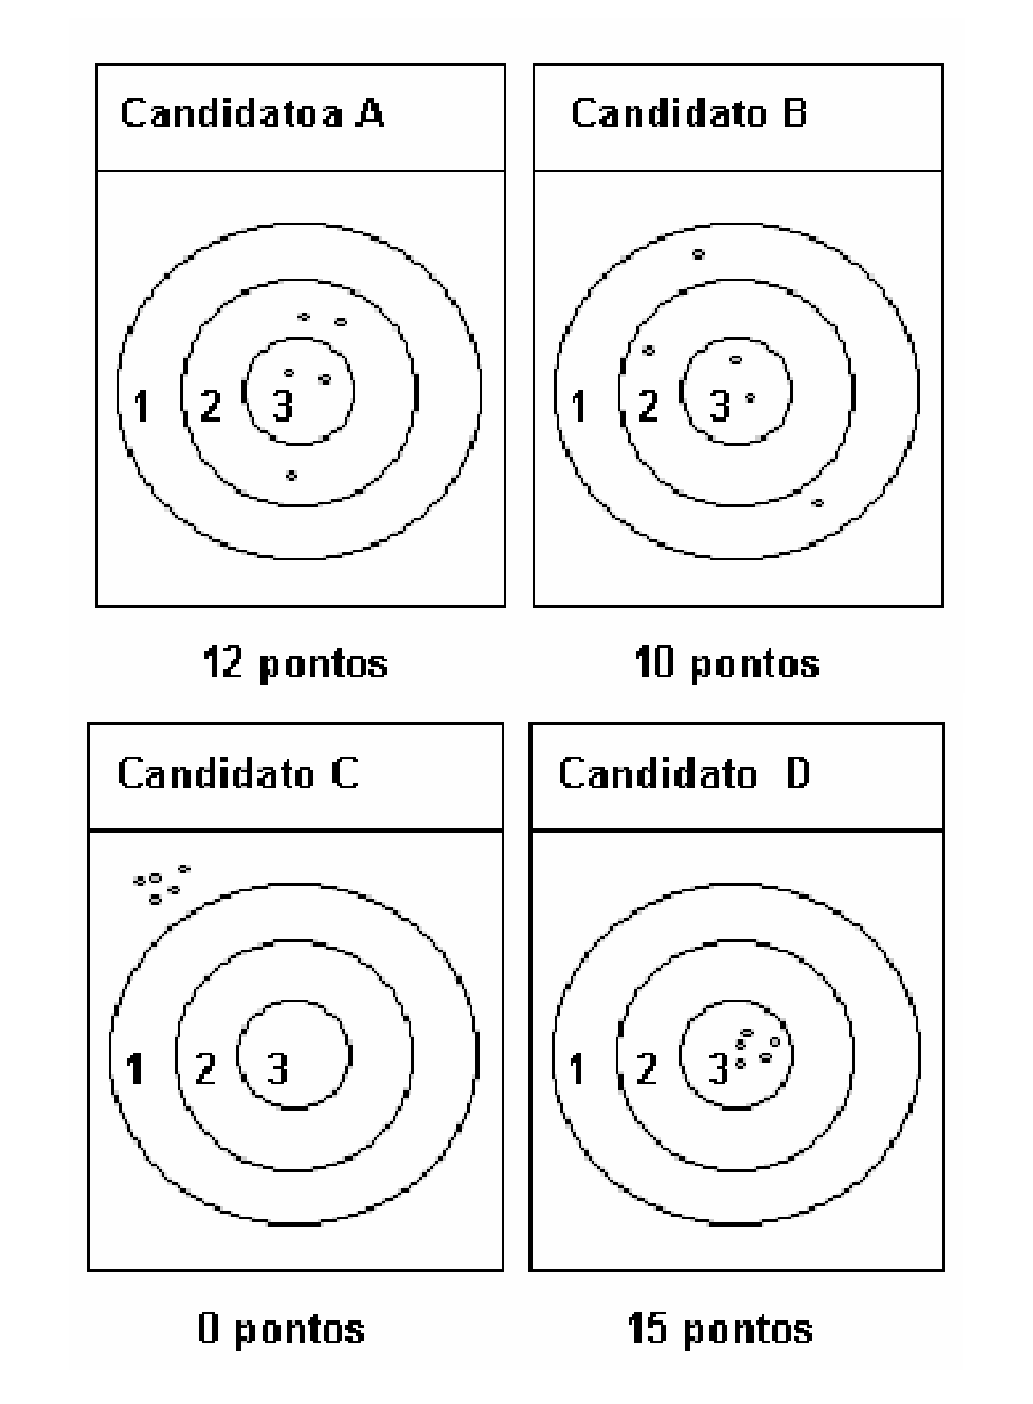
\includegraphics[scale=0.6]{figures/disp.eps}\\
  \vspace{-0.6cm}
  \caption{Exemplo Prático sobre Dispersão ou Variabilidade dos Dados}\label{esquematabela}
  }
\end{figure}

\newpage

O candidato mais "eficiente", em principio, deve corresponder àquele que tiver a maior média de pontos por tiro, o que nos conduz ao candidato D, que obteve uma média de 15/5 = 3 pontos/tiro.  Entretanto, verifica-se com uma simples inspeção dos alvos mostrados que o ("vesguinho") candidato C tem alguma chance de se constituir em um bom representante, mesmo com média de 0 pontos/tiro, após corrigirmos defeitos de sua visão, uma vez que ele mostrou ter uma pontaria muito "certeira"(!).  Pelos exemplos mostrados acima, vemos a necessidade de medidas complementares, visando a uma melhor análise da dispersão ou variabilidade dos resultados numéricos.\vskip0.3cm



Todas as medidas citadas têm um mesmo objetivo principal, ou seja, a quantificação da dispersão ou homogeneidade dos elementos das séries, permitindo dessa forma a comparação entre as mesmas no que a isso diz respeito. A série mais homogênea de todas é aquela cujos elementos são todos iguais entre si, o que nos leva à nulidade de todas as medidas de dispersão citadas acima. Observou-se dessa forma que, tão homogênea quanto à equipe de futebol que vence todas as partidas que disputa, é a equipe que perde também todas as suas partidas. Pode-se, em princípio, afirmar que, entre duas ou mais séries, a mais homogênea (ou menos dispersa) é aquela que apresenta a menor medida de dispersão, medida essa escolhida convenientemente.\vskip0.3cm

Em suma, o grau aos quais os dados numéricos tendem a dispersar-se em torno de um valor médio chama-se variação ou dispersão dos dados. Elas permitem se identificar até que ponto os resultados se concentram ou não ao redor da tendência central de um conjunto de observações.\vskip0.3cm

Dispõe-se de várias medidas de dispersão ou de variação, sendo as mais comuns, a amplitude total, o desvio médio, a amplitude semi-interquartílica, a variância, o desvio padrão, o erro padrão e o coeficiente de variação, cada um expressando diferentes formas de se quantificar a tendência que os resultados de um experimento aleatório têm de se concentrarem ou não em determinados valores (quanto maior a dispersão, menor a concentração e vice-versa).




\subsection{Desvio Médio (DM)}

\begin{equation}\label{dn}
    DM= \left[  \frac{\sum_{i=1}^{n}|(x_{i}-\bar{X})|}{n} \right]
\end{equation}

\newpage 

\subsection{Variância ($S^{2}$) de Dados Brutos}

A variância amostral de um conjunto de dados $x_{1},x_{2},\ldots,x_{n}$ , é assim definida:

\begin{eqnarray}\nonumber
S^{2} = \left[ \frac{(x_{1}-\bar{X})^{2}+(x_{2}-\bar{X})^{2}+\ldots+(x_{n}-\bar{X})^{2}}{n-1} \right]
    & = &  \\
    \left[ \frac{\sum_{i=1}^{n}(x_{i}-\bar{X})^{2}}{n-1} \right]  & = &  \\ \nonumber
    \left[ \frac{\sum_{i=1}^{n}x_{i}^{2}-\frac{(\sum_{i=1}^{n}x_{i})^{2}}{n}}{n-1} \right] &  &
\end{eqnarray}


\subsection{Variância ($S^{2}_{t}$) de Dados Tabulados}


\begin{eqnarray}\nonumber
S^{2} = \left[ \frac{(x_{1}-\bar{X})^{2}f_{1}+(x_{2}-\bar{X})^{2}f_{2}+\ldots+(x_{n}-\bar{X})^{2}f_{n}}{n-1} \right]
    & = &  \\
    \left[ \frac{\sum_{i=1}^{n}(x_{i}-\bar{X})^{2}f_{i}}{n-1} \right]  & = &  \\ \nonumber
    \left[ \frac{\sum_{i=1}^{n}x_{i}^{2}f_{i}-\frac{(\sum_{i=1}^{n}x_{i}f_{i})^{2}}{n}}{n-1} \right] &  &
\end{eqnarray}



\subsection{Variância Aparada ($S_{\alpha}^{2}$)}

Uma medida ainda mais elaborada de dispersão é conhecida como "Variância Aparada" (trimmed variance). A idéia, como para a "média aparada", é omitir uma proporção dos maiores e menores valores e calcular o análogo da variância amostral:

\begin{equation}\label{varAparada}
    S_{\alpha}^{2} = \left[\frac{1}{n-2k}\right]\sum_{i=k+1}^{n-k}(X_{i}-\bar{X}_{\alpha})^{2}
\end{equation}


Onde k é o inteiro mais próximo de $\alpha n$. Veja que é feita a média do quadrado dos desvios entre o valor e as médias aparadas consistentes (de acordo com a \label{aparada}). A variância aparada é algumas vezes multiplicada por um fator de ajuste para fazê-la mais consistente com a variância amostral ($S^{2}$).


\subsection{Desvio Padrão (DP)}

Definido como a raiz quadrada positiva da variância, o desvio-padrão exerce grande vantagem sobre a variância, já que ele é apresentado na mesma unidade de medida dos dados brutos. Trata-se da mais importante das medidas de variabilidade, onde indica a dispersão média absoluta dos dados em torno da própria média aritmética. O desvio-padrão pode ser assim obtido de duas maneiras:\vskip0.3cm

Para dados brutos, dp será

\begin{equation}\label{dp}
    DP= \sqrt{\frac{\sum_{i=1}^{n}(x_{i}-\bar{X})^{2}}{n-1}} = \sqrt{S^{2}}
\end{equation}

Já para dados tabulados, ficará

\begin{equation}\label{dp}
    DP= \sqrt{\frac{\sum_{i=1}^{n}(x_{i}-\bar{X})^{2}f_{i}}{n-1}} = \sqrt{S^{2}}
\end{equation}

\subsection{Coeficiente de Variação (CV)}

O coeficiente de variação é uma medida de dispersão relativa, e útil para comparação, em termos relativos, do grau de concentração, em torno da média, de séries distintas. Pó ser um número adimensional permite a comparação de séries de variáveis com unidades diferentes. Assim, o CV é a razão percentual entre o desvio padrão e a média aritmética, ou seja, pode-se caracterizar a dispersão ou variabilidade dos dados em termos relativos ao seu valor médio, sendo representada por:


\begin{equation}\label{CV}
    CV= \left[ \frac{S}{\bar{X}} \right]*100
\end{equation}

\newpage

\section{Medidas de Ordenação ou Separatrizes}
\subsection{Quartis $(Q_{i})$}






Quartis são medidas que dividem (separam) uma amostra (ou coleção) de dados de tipo quantitativo (ou qualitativo ordinal) ordenada em 4 partes iguais (FEIJOO, 2010).



\begin{enumerate}
  \item[{1)}] O 1º Quartil ou quartil inferior, representado por ($Q_{1}$) ou ($Q_{0,25}$), é o valor tal que pelo menos 25\% dos dados são não maiores do que ele e pelo menos 75\% dos dados são não menores do que ele;


  
  \item[{2)}] No 2º Quartil ($Q_{2}$), 50\% dos elementos estarão abaixo dele e 50\%, acima. Observe então que o 2º Quartil é igual à Mediana.
  \item[{3)}] No 3º Quartil ($Q_{3}$), 75\% dos elementos estarão abaixo dele e 25\%, acima.
  \vskip0.3cm
 \item[{4)}] No 4º Quartil ($Q_{4}$), 100\% dos elementos estarão resumidos. Nota-se que o 4º quartil é igual a média artimética.
\end{enumerate}


Para o cálculo do quartil utilizam-se os seguintes passos.



\begin{enumerate}

\item [{1°)}] Ordena-se os dados do menor para o maior;
\item [{2°)}] Encontra-se a frequência acumulada da distribuição;
\item [{3°)}]Calcula-se a posição do quartil na tabela.
$$ P_{(q_{i})} = \left[ \frac{(i \times n)}{4}  \right] $$
\item [{4°)}] Posteriormente, marca-se na tabela a posição pela frequência acumulada, para identificar em qual classe estará o quartil.
\item [{5°)}] Em seguida aplica-se a fórmula do quartil
\end{enumerate}

\begin{equation}\label{}
    Q_{1}= l_{q_{i}}+\left[\frac{P_{i}-FAA}{f_{q_{1}}}\right]\times h_{1}
\end{equation}

 onde

 \begin{itemize}
   \item $l_{q_{i}}=$ é o limite inferior da classe do quartil de ordem i;
   \item $FAA=$ È a freqüência acumulada anterior da classe do quartil de ordem i;
   \item $f_{q_{i}}=$ È a freqüência simples da classe do quartil de ordem i;
   \item $h_{i}=$ é o intervalo de classe;
 \end{itemize}




\subsection{Decis $(D_{i})$}

Dividem uma Distribuição de freqüência em 10 partes iguais.


\begin{enumerate}
  \item[{1)}] No $1º$ Decil ($D_{1}$), 10\% dos elementos estarão abaixo dele e 90\%, acima.
  \item[{2)}] No $2º$ Decil ($D_{2}$), 20\% dos elementos estarão abaixo dele e 80\%, acima.
  \item[{3)}] No $3º$ Decil ($D_{3}$), 30\% dos elementos estarão abaixo dele e 70\%, acima.
  \item[{4)}] $\ldots \ldots \ldots \ldots \ \ \  \ldots \ldots \ldots \ldots \ \ \  \ldots \ldots \ldots \ldots \ \ \  \ldots \ldots \ldots \ldots \ \ \ldots \ldots \ldots \ldots$
 \item[{5)}] No $10º$ Decil ($D_{10}$), 100\% dos elementos estão resumidos. Observe então que o $10º$ decil é igual a média artimética.
\end{enumerate}

\begin{enumerate}
\item [{1)}]Calcula-se primeira a posição do decil na tabela.
$$ P_{(d_{i})} = \left[ \frac{(i \times n)}{10} \right] $$
\item [{2)}] Posteriormente, marca-se na tabela a posição pela frequência acumulada, para identificar em qual classe estará o decil.
\item [{3)}] Em seguida aplica-se a fórmula do decil
\end{enumerate}

\begin{equation}\label{}
    D_{1}= l_{d_{i}}+\left[\frac{P_{d_{i}}-FAA}{f_{d_{1}}}\right]\times h_{1}
\end{equation}

 onde

 \begin{itemize}
   \item $l_{d_{i}}=$ é o limite inferior da classe do decil de ordem i;
   \item $FAA=$ È a freqüência acumulada anterior da classe do decil de ordem i;
   \item $f_{d_{i}}=$ È a freqüência simples da classe do decil de ordem i;
   \item $h_{i}=$ é o intervalo de classe;
 \end{itemize}



\subsection{Percentis $(P_{i})$}

Dividem uma Distribuição de freqüência em 100 partes iguais. Então:


\begin{enumerate}
  \item[{1)}] No $1º$ Percentil ($P_{1}$), 1\% dos elementos estarão abaixo dele e 99\% estarão acima.
  \item[{2)}] No $2º$ Percentil ($P_{2}$), 2\% dos elementos estarão abaixo dele e 98\% estarão acima.
  \item[{3)}] No $3º$ Percentil ($P_{3}$), 3\% dos elementos estarão abaixo dele e 97\% estarão acima.
   \item[{4)}] $\ldots \ldots \ldots \ldots \ \ \  \ldots \ldots \ldots \ldots \ \ \  \ldots \ldots \ldots \ldots \ \ \  \ldots \ldots \ldots \ldots \ \ \ldots \ldots \ldots \ldots$
  \item[{5)}] No $99º$ Percentil ($P_{99}$), 99\% dos elementos estarão abaixo dele e 1\% estarão acima.
   \item[{6)}] No $100º$ Percentil ($P_{100}$), 100\% dos elementos estão resumidos. Observe então que o $100º$ Percentil é igual a média artimética.
\end{enumerate}



\begin{enumerate}
\item [{1)}]Calcula-se primeira a posição do percentil na tabela.
$$ P_{(p_{i})} = \left[ \frac{(i \times n)}{100} \right] $$
\item [{2)}] Posteriormente, marca-se na tabela a posição pela frequência acumulada, para identificar em qual classe estará o percentil.
\item [{3)}] Em seguida aplica-se a fórmula do percentil
\end{enumerate}

\begin{equation}\label{}
    P_{p_{i}}= l_{p_{i}}+\left[\frac{P_{p_{i}}-FAA}{f_{p_{i}}}\right]\times h_{1}
\end{equation}

 onde

 \begin{itemize}
   \item $l_{p_{i}}=$ é o limite inferior da classe do percentil de ordem i;
   \item $FAA=$ È a freqüência acumulada anterior da classe do percentil de ordem i;
   \item $f_{p_{i}}=$ È a freqüência simples da classe do percentil de ordem i;
   \item $h_{i}=$ é o intervalo de classe;
 \end{itemize}



\section{Medidas de Forma, Enviesamento ou Assimetria }

\inic Embora sejam menos utilizadas na prática que as medidas de posição e
dispersão, as medidas de assimetria (\textit{skewness}) e curtose são úteis para
identificar modelos probabilísticos para análise inferencial.

\inic As medidas de assimetria e curtose são as que restam para complementarmos o quadro das estatísticas descritivas, que proporcionam, juntamente com as medidas de posição e de dispersão, a descrição e compreensão completas da distribuição de freqüências estudadas.\vskip0.3cm

Assimetria, como próprio nome insinua, significa desvio ou afastamento, ou seja, é o grau de desvio da simetria de uma distribuição ou afastamento de informação de uma curva de freqüência.\vskip0.3cm




%$$ b=\frac{1}{n}\sum_{i=1}^{n}\left[\frac{x_{i}-\bar{X}}{s}\right]^{2} $$

Uma medida usada muito freqüentemente para avaliar o grau de assimetria ou de deformação de uma distribuição e o coeficiente sugerido por Karl Pearson, o qual se calcula mediante as seguintes expressões:

\begin{enumerate}
  \item [{1)}]Primeiro Coeficiente de Assimetria de Pearson
  \begin{equation}\label{assimetria}
    AS = \left[ \frac{(Media-Moda)}{(Desvio-Padrao)} \right] = \left[  \frac{(\bar{X}-M_{o})}{S_{x}} \right]
\end{equation}
  \item [{2)}]Segundo Coeficiente de Assimetria de Pearson
  \begin{equation}\label{assimetria}
    AS = \left[ \frac{(Q_{3}+Q_{1}-2M_{e})}{(Q_{3}-Q_{1})} \right]
\end{equation}
    ou
 \begin{equation}
    AS = \left[ \frac{3(\bar{X}-M_{e})}{S_{x}} \right]
\end{equation}
\end{enumerate}






\textbf{Escala de Assimetria}

\begin{enumerate}
\item $|AS| =0$ a distribuição é Simétria
\item $|AS| < 0,15$ a Assimetria é Pequena
\item $0,15 < |AS| <1$ a Assimetria é Moderada
\item $|AS| > 1$ a Assimetria é Elevada
\end{enumerate}


\newpage 

Em um conjunto de dados, a mediana, a moda e a média
não necessariamente devem apresentar o mesmo valor. Uma
informação importante é que a mediana não é influenciada pelos valores extremos. Comparando os resultados encontrados para uma amostra em relação às medidas de posição estudadas e verificando a inter-relação entre elas, você pode concluir que seus valores podem nos dar um indicativo da natureza da distribuição dos dados, em função das regras definidas a seguir:


\begin{itemize}
\item Se a $\bar{X}=media$ for maior que a $\tilde{X}=mediana$ e maior que a Moda então a distribuição é assimétrica a direita (positiva), ou seja, os dados estão mais concentrados a direita.  	
\item Se a $\bar{X}$ for igual a $\tilde{X}$ e igual a moda então a distribuição é simétrica.
\item Se a $\bar{X}= media$ for menor que a $\tilde{X}= mediana$ e menor que a Moda então a distribuição é assimétrica a esquerda (negativa), ou seja, os dados estão mais concentrados a esquerda. 	
\end{itemize}

As medidas de tendência  central possuem algumas vantagens e desvantagens. A média possue a vantagem de Refletir cada valor observado na distribuição, e a desvantagem de ser influenciada por valores extremos. Já a mediana é menos sensível a valores extremos do que a Média, porém, é Difícil de determinar para grande quantidade de dados. Enquanto que a moda tem maior quantidade de valores concentrados neste ponto, e não se presta a análise matemática.
 
\newpage 

\section{Medidas de Achatamento, Afilamento ou Curtose }

\inic Em alguns casos uma distribuição pode ter seus valores concentrados próximos da média tal que a distribuição tem um pico mais alto, em outros casos a distribuição pode ser plana. Assim, medidas do grau de agudez de uma distribuição são chamadas de coeficiente de curtose (SPIGEL et al, 2013). \vskip0.3cm

\inic A curtose ou excesso indica até que ponto a curva de freqüências de uma distribuição se apresenta mais afilada ou mais achatada do que uma curva-padrão, denominada curva normal.\vskip0.3cm

\inic A medida de curtose é o grau de achatamento de uma distribuição, considerando usualmente em relação a uma distribuição normal. De acordo com o grau de curtose, podemos ter três tipos de curvas de freqüência: \textbf{Mesocúrtica}, \textbf{Leptocúrtica} e \textbf{Platicúrtica}.\vskip0.3cm

\begin{itemize}
\item Quando a distribuição apresenta uma curva de frequência mais fechada (mais aguda em sua parte superior), ela é denominada Leptocúrtica (Lepto = Delgado, Alongado, Magro, etc).
\item A distribuição de referência (Distribuição Normal) é denominada Mesocúrtica (Meso = Meio, Central, etc).
\item Quando a distribuição apresenta uma curva de frequência mais aberta (mais achatada em sua parte superior), ela é denominada Platicúrtica (Plato = Chato, Plano, Largo, etc).
\end{itemize}

Para avaliar o grau de curtose de uma curva ou distribuição de freqüências, usa-se o Coeficiente Percentílico de Curtose (K):

\begin{equation}\label{curtose}
    K = \left[ \frac{(Q_{3}-Q_{1})}{2(D_{9}-D_{1})} \right]
\end{equation}

Onde

\begin{itemize}
  \item $Q_{1}$ e $Q_{3}$  = é o primeiro e terceiro quartil;
  \item $D_{1}$ e $D_{9}$  = é o primeiro e nono decil;
   \end{itemize}

\vskip0.3cm

Sendo que existe um caso particular e a fórmula \ref{curtose} pode ser substituída
pelos percentis $P_{90}=D_{9}$ e $P_{10}=D_{1}$, quando for o caso.




\vskip0.3cm
Uma outra forma de representar o coeficiente de Curtose é da seguinte maneira

\begin{equation}\label{curtose2}
    K= \left[ \frac{C}{D_{9}-D_{1}} \right]
\end{equation}

onde o C é chamado de amplitude semi-interquartilica

\begin{equation}\label{curtose2}
    C= \left[ \frac{Q_{3}-Q_{1}}{2} \right]
\end{equation}


\textbf{Escala de Curtose}

\begin{enumerate}
\item Se $K = 0,263 \Rightarrow$  A curva correspondente à distribuição de frequências é \textbf{Mesocúrtica};
\item Se $K < 0,263 \Rightarrow$  A curva correspondente à distribuição é concentrada ao redor da média, ou seja, é mais pontiaguda ou afunilada e menos dispersa, sendo classificada de \textbf{Leptocúrtica};
\item Se $K > 0,263 \Rightarrow$ A curva correspondente à distribuição de frequência é mais dispersa ou Achatada, classificada de \textbf{Platicúrtica};
\end{enumerate}
